\documentclass[a4paper, 11pt]{article} % Font size (can be 10pt, 11pt or 12pt) and paper size (remove a4paper for US letter paper)

\usepackage[protrusion=true,expansion=true]{microtype} % Better typography
\usepackage[a4paper, margin=3.5cm]{geometry} %Annina style
\usepackage{graphicx} % Required for including pictures
\usepackage{wrapfig} % Allows in-line images
\usepackage{enumitem} %%Enables control over enumerate and itemize environments
\usepackage{setspace}
\usepackage{amssymb,amsmath,mathrsfs,amsthm} %%Math packages
\usepackage{stmaryrd}
\usepackage{mathtools}
\usepackage{mathpazo} % Use the Palatino font
\usepackage[T1]{fontenc} % Required for accented characters
\usepackage{array}
\usepackage{bibentry}
\usepackage[round]{natbib} %%Or change 'round' to 'square' for square backers
% \usepackage{tikz}
\usepackage{comment}

\usepackage{lipsum}
\newenvironment{Answer}[1][Answer]
  {\proof[#1]\leftskip=1cm\rightskip=1cm}
  {\endproof}
  % \def\firstcircle{(140:-1.5cm) circle (1.5cm)}
  % \def\secondcircle{(210:1.75cm) circle (2.5cm)}
  % \def\thirdcircle{(330:1.75cm) circle (2.5cm)}


\setcitestyle{aysep={}}

\linespread{1.05} % Change line spacing here, Palatino benefits from a slight increase by default

\renewcommand{\qed}[0]{$\hfill\Box$} %%Box at end of proofs
\newcommand{\s}[0]{\mathcal{S}} %%Box at end of proofs
\renewcommand{\L}[0]{\mathcal{L}} %%Box at end of proofs
\newcommand{\V}[0]{\mathcal{V}} %%Box at end of proofs
\renewcommand{\t}[0]{\mathcal{A}} %%Box at end of proofs
\newcommand{\corner}[1]{\ulcorner#1\urcorner} %%Corner quotes
\newcommand{\tuple}[1]{\langle#1\rangle} %%Angle brackets
\newcommand{\set}[1]{\lbrace#1\rbrace} %%Set brackets
\newcommand{\interpret}[1]{\llbracket#1\rrbracket} %%Double brackets
%\DeclarePairedDelimiter\ceil{\lceil}{\rceil}    
\newcommand{\qpar}[0]{\par\hspace*{.2in}}


\newtheorem{innercustomthm}{}
\newenvironment{customthm}[1]
  {\renewcommand\theinnercustomthm{#1}\innercustomthm}
  {\endinnercustomthm}


\newtheoremstyle{theorem}
{}                % Space above
{}                % Space below
{\normalfont}        % Theorem body font % (default is "\upshape")
{}                % Indent amount
{\bfseries}       % Theorem head font % (default is \mdseries)
{}               % Punctuation after theorem head % default: no punctuation
{.18in}               % Space after theorem head
{}                % Theorem head spec
\theoremstyle{theorem}
\newtheorem{theorem}{}% theorem counter resets every \subsection
\renewcommand{\thetheorem}{T\arabic{theorem}}% Remove subsection from theorem counter representation


\newtheoremstyle{Pthm}
{}                % Space above
{}                % Space below
{\normalfont}        % Theorem body font % (default is "\upshape")
{.25in}                % Indent amount
{\bfseries}       % Theorem head font % (default is \mdseries)
{}               % Punctuation after theorem head % default: no punctuation
{.18in}               % Space after theorem head
{}                % Theorem head spec
\theoremstyle{Pthm}
\newtheorem{Pthm}{}% theorem counter resets every \subsection
\renewcommand{\thePthm}{P\arabic{Pthm}}% Remove subsection from theorem counter representation


\usepackage{calc}
\makeatletter
\newcommand{\labelalign@original@item}{}
\let\labelalign@original@item\item
\newcommand*{\labelalign@envir}{labelalign}
\newlength{\labelalign@totalleftmargin}
\newlength{\labelalign@linewidth}
\newcommand{\labelalign@makelabel}[1]{\llap{#1}}%
\newcommand{\labelalign@item}[1][]{%
  \setlength{\@totalleftmargin}%
       {\labelalign@totalleftmargin+\widthof{\textbf{#1 }}+.25in-\leftmargin}%
  \setlength{\linewidth}
       {\labelalign@linewidth-\widthof{\textbf{#1 }}-.25in+\leftmargin}%
  \par\parshape \@ne \@totalleftmargin \linewidth
  \labelalign@original@item[\textbf{#1}]%
}
\newenvironment{labelalign}
  {\list{}{\setlength{\labelwidth}{0in}%
           \let\makelabel\labelalign@makelabel}%
   \setlength{\labelalign@totalleftmargin}{\@totalleftmargin}%
   \setlength{\labelalign@linewidth}{\linewidth}%
   \renewcommand{\item}{\ifx\@currenvir\labelalign@envir
                           \expandafter\labelalign@item
                        \else
                           \expandafter\labelalign@original@item
                        \fi}}
  {\endlist}
\makeatother


\makeatletter
\renewcommand\@biblabel[1]{\textbf{#1.}} % Change the square brackets for each bibliography item from '[1]' to '1.'
\renewcommand{\@listI}{\itemsep=0pt} % Reduce the space between items in the itemize and enumerate environments and the bibliography

\lineskiplimit=-100pt\relax

\renewcommand{\maketitle}{ % Customize the title - do not edit title and author name here, see the TITLE block below
\begin{flushright} % Right align
{\LARGE\@title} % Increase the font size of the title

\vspace{10pt} % Some vertical space between the title and author name

{\@author} % Author name
\\\@date % Date

\vspace{30pt} % Some vertical space between the author block and abstract
\end{flushright}
}

%----------------------------------------------------------------------------------------
%	TITLE
%----------------------------------------------------------------------------------------

\title{\textbf{Revisions: TT2021}} % Subtitle

\author{\textsc{Introduction to Logic}\\ \em Benjamin Brast-McKie} % Institution

\date{\today} % Date

%----------------------------------------------------------------------------------------

\begin{document}

\maketitle % Print the title section

\thispagestyle{empty}

%------------------------------------------------------------------------


% \section*{TT2020: Problem 1}

% \begin{center}
%   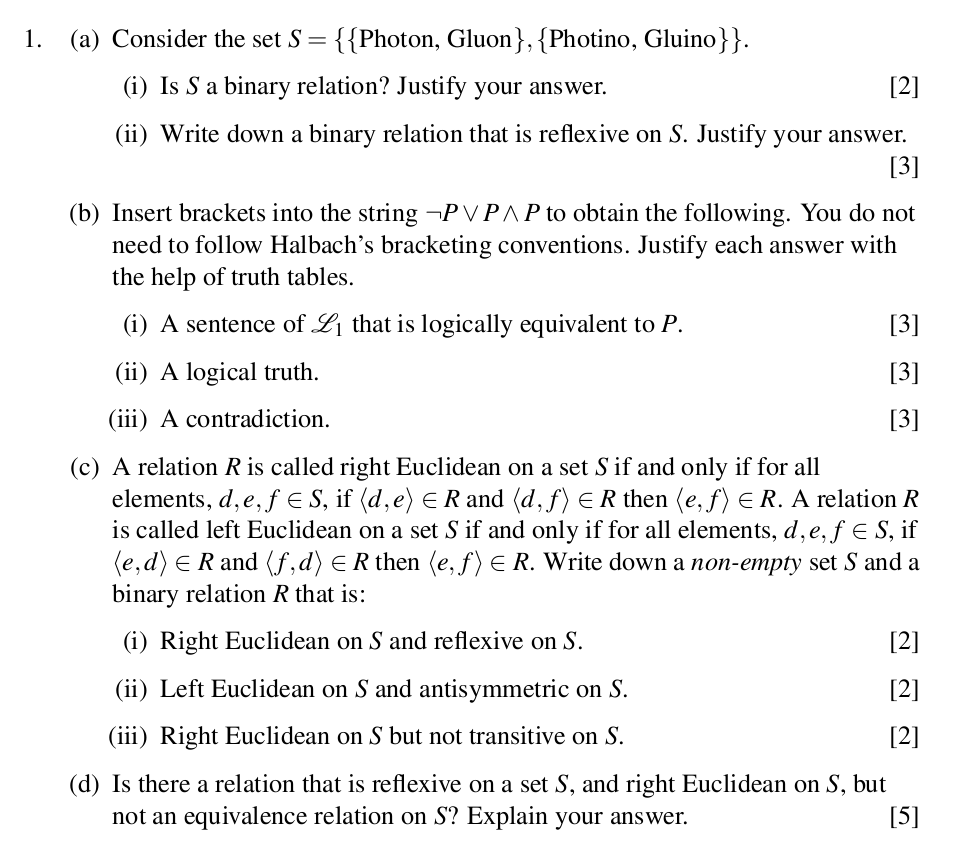
\includegraphics[width=1\textwidth]{Problem1.png}
% \end{center}



% \section*{Solutions}



% \vspace{.1in}
% \begin{customthm}{(1.a.ii)}
%   Write down a binary relation that is reflexive on S.
% \end{customthm}

% \begin{Answer}
% $R=\set{\tuple{\set{\text{Photon},\text{Gluon}},\set{\text{Photon},\text{Gluon}}},\tuple{\set{\text{Photino},\text{Gluino}},\set{\text{Photino},\text{Gluino}}}}$
% \end{Answer}

% \newpage

% \vspace{.1in}
% \begin{customthm}{(1.b)}
%   Insert brackets into the string $\neg P\vee P\wedge P$.
% \end{customthm}

% \begin{Answer}
%   (i) $(\neg P\vee P)\wedge P$; 
%   (ii) $\neg P\vee(P\wedge P)$; 
%   (iii) $\neg(P\vee P)\wedge P$.
% \end{Answer}



% \vspace{.1in}
% \begin{customthm}{(1.c)}
%   Write down a non-empty set $S$ and a binary relation $R$.
% \end{customthm}

% \begin{Answer}
%   (i) $S=\set{1},\ R=\set{\tuple{1,1}}$;
%   % (ii) $S=\set{1,2,3}$,\ $R=\set{\tuple{1,2},\tuple{3,2},\tuple{1,3},\tuple{3,1}}$
%   (ii) $S=\set{1,2},\ R=\varnothing$;\\
%   % (iii) $S=\set{1,2},\ R=\set{\tuple{1,1},\tuple{2,1},\tuple{1,2}}$
%   % (iii) $S=\set{1},\ R=\set{}$
%   (iii) $S=\set{1,2,3}$,
%   $R=\set{\tuple{1,2},\tuple{2,3},\tuple{2,2},\tuple{3,2},\tuple{3,3}}$.
% \end{Answer}




% \vspace{.1in}
% \begin{customthm}{(1.d)}
%   Is there a relation that is reflexive on a set $S$, and right Euclidean on $S$, but not an equivalence relation on $S$?
% \end{customthm}

% \begin{Answer}
%   % $S=\set{1,2},\ R=\set{\tuple{1,2},\tuple{1,1},\tuple{2,2},\tuple{2,1}}$
%   No.
%   Assume that $R$ is any relation which is reflexive and right Euclidean on $S$.
%   We must show that $R$ is also symmetric and transitive on $S$ in order to establish that $R$ is an equivalence relation on $S$.

%   \textit{Symmetry:} Assume that $R$ is non-symmetric on $S$.
%   Thus there are some $x,y\in S$ where $\tuple{x,y}\in R$, but $\tuple{y,x}\notin R$.
%   By reflexivity, $\tuple{x,x}\in R$, and so $\tuple{y,x}\in R$ since $R$ is right Euclidean on $S$, contradicting our case assumption.
%   Thus $R$ is symmetric on $S$.

%   \textit{Transitivity:} Assume that $R$ is non-transitive on $S$.
%   Thus there are some $x,y,z\in S$ where $\tuple{x,y},\tuple{y,z}\in R$, but $\tuple{x,z}\notin R$.
%   % Since $R$ is reflexive on $S$, then $\tuple{x,x},\tuple{y,y},\tuple{z,z}\in R$
%   By symmetry, we know that $\tuple{y,x}\in R$, and so $\tuple{x,z}\in R$ since $R$ is right Euclidean on $S$, contradicting our case assumption.
%   Thus $R$ is transitive on $S$.
% \end{Answer}







% \section*{TT2020: Problem 2}

% \begin{center}
%   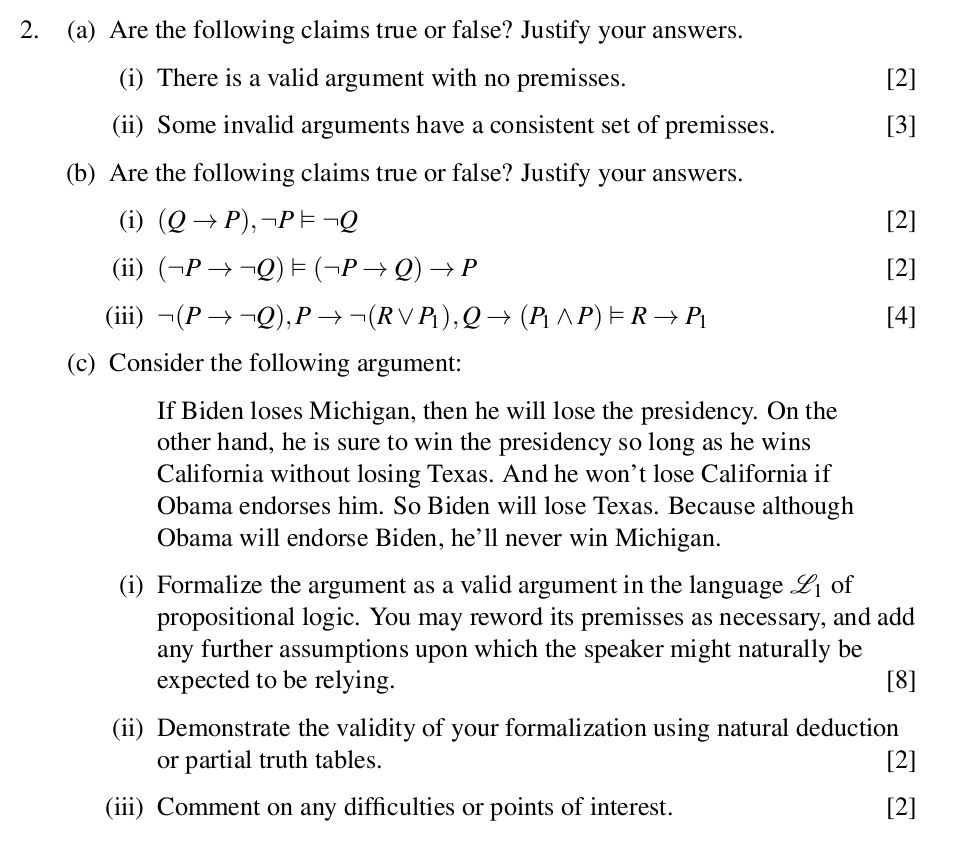
\includegraphics[width=1\textwidth]{Problem2.png}
% \end{center}



% \section*{Solutions}



% \vspace{.1in}
% \begin{customthm}{(2.a.i)}
%   There is a valid argument with no premisses.
% \end{customthm}

% \begin{Answer}
%   True, for instance $\vDash P\vee\neg P$.

%   Assume for contradiction that there is an $\mathscr{L}_1$ structure $A$ where $|P\vee\neg P|_A=F$.
%   Thus $|P|_A=F$ and $|\neg P|_A=F$, and so both $|P|_A=F$ and $|P|_A=T$, which is a contradiction.
%   It follows that there is no $\mathscr{L}_1$ structure $A$ where $|P\vee\neg P|_A=F$, and so the argument is valid.
% \end{Answer}


% % \vspace{.1in}
% % \begin{customthm}{(2.b.i)}
% %   $Q\rightarrow P, \neg P$
% % \end{customthm}

% % \begin{Answer}
  
% % \end{Answer}



% \vspace{.1in}
% \begin{customthm}{(2.b.ii)}
%   $\neg P\rightarrow\neg Q\vDash(\neg P\rightarrow Q)\rightarrow P$
% \end{customthm}

% \begin{Answer}
%   Assume for contradiction that there is some structure $A$ where: (1) $|\neg P\rightarrow\neg Q|_A=T$; and (2) $|(\neg P\rightarrow Q)\rightarrow P|_A=F$.
%   It follows from (2) that: (3) $|\neg P\rightarrow Q|_A=T$; and (4) $|P|_A=F$.

%   By (1), either $|\neg P|_A=F$ or $|\neg Q|_A=T$, and so either $|P|_A=T$ or $|Q|_A=F$.
%   Thus $|Q|_A=F$ follows by (4).
%   Since $|\neg P|_A=T$ also follows by (4), we may conclude that $|\neg P\rightarrow Q|_A=F$ contradicting (3).

%   It follows that there is no structure $A$ which makes the premise true and the conclusion false, and so the argument is valid.
% \end{Answer}







\vspace{-50pt}


\section*{TT2020: Problem 3}

\begin{center}
  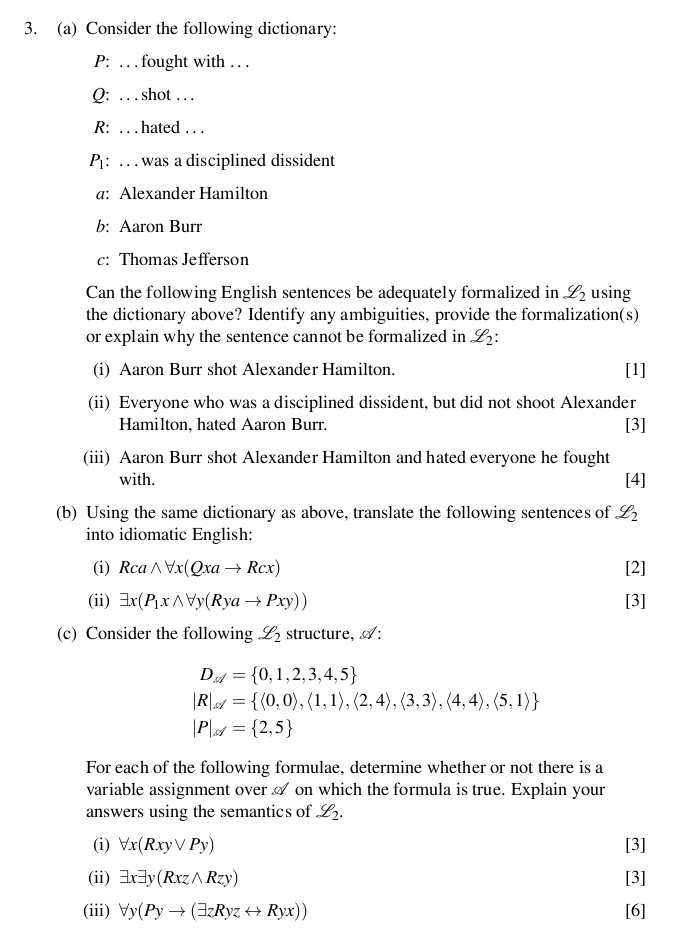
\includegraphics[width=1\textwidth]{Problem3.png}
\end{center}



\section*{Solutions}

\vspace{.1in}
\begin{customthm}{(3.a)}
  Formalise (i) -- (iii) in $\mathscr{L}_2$.
\end{customthm}

\begin{Answer}
  % (ii) $\forall x[(P_1x\wedge\neg Qxa)\rightarrow Rxb]$; 
  % (iii) $Qba\wedge\forall x(Pbx\rightarrow Rbx)$.\\
  % (iii)$^*$  $Qba\wedge\forall x(Pax\rightarrow Rbx)$.
\end{Answer}




\vspace{.1in}
\begin{customthm}{(3.b)}
  Translate from $\mathscr{L}_2$ into idiomatic English.
\end{customthm}

\begin{Answer}
  % (i)$^*$ Thomas Jefferson hated Alexander Hamilton and for all $x$, if $x$ shot Thomas Jefferson, then Thomas Jefferson hated $x$;
  % (i) Thomas Jefferson hated Alexander Hamilton and everyone who shot him;
  % (ii) There was a disciplined dissident who fought with everyone who hated Alexander Hamilton.
\end{Answer}





\vspace{.1in}
\begin{customthm}{(3.c)}
  Determine whether there is a variable assignment over $A$ on which the formula is true using the semantics of $\mathscr{L}_2$.
\end{customthm}

\begin{Answer}
  % (i) Yes.
  %   Let $a$ be a v.a. where $|y|_A^a=2$.
  %   It follows that $|P_y|_A^a=T$ since $2\in|P|_A$.
  %   By the semantics for disjunction, $|Rxy\vee P_y|_A^a=T$ independent of what $|x|_A^a$ happens to be.
  %   Thus $|Rxy\vee P_y|_A^b=T$ for any v.a. $b$ differing at most from $a$ in $x$, and so $|\forall x(Rxy\vee P_y)|_A^a=T$ for some v.a. $a$ over $A$.
\end{Answer}



\begin{Answer}
  % (ii) Yes.
  %   Let $a$ be a v.a. where $|x|_A^a=2$, $|y|_A^a=4$, and $|z|_A^a=4$. 
  %   Observe that both $|Rxz|_A^a=|Rzy|_A^a=T$, and so $|Rxz\wedge Rzy|_A^a=T$ by the semantics for conjunction.
  %   Since $a$ is a v.a. which differs at most from $a$ (in this case itself) in $y$ where $|Rxz\wedge Rzy|_A^a=T$, we know that $|\exists y(Rxz\wedge Rzy)|_A^a=T$.
  %   Similarly, since $a$ is a v.a. differing at most from itself in $x$ where $|\exists y(Rxz\wedge Rzy)|_A^a=T$, we may conclude that $|\exists x\exists y(Rxz\wedge Rzy)|_A^a=T$ as desired.
\end{Answer}


\begin{Answer}
  % (iii) No.
  %   Assume otherwise for contradiction.
  %   It follows that $|\forall y[Py\rightarrow(\exists zRyz\leftrightarrow Ryx)]|_A^a=T$ for some v.a. $a$ over $A$. 
  %   We may then conclude that $|Py\rightarrow(\exists zRyz\leftrightarrow Ryx)|_A^b=T$ for any v.a. $b$ differing at most from $a$ in $y$ by the semantics for universal generalisation.

  %   In particular, let $b$ be a v.a. differing at most from $a$ in that $|y|_A^b=2$. 
  %   It follows that $|Py|_A^b=T$ since $|y|_A^b\in|P|_A$, and so by the semantics for the conditional, $|\exists zRyz\leftrightarrow Ryx|_A^b=T$.

  %   We may then let $c$ be a v.a. differing at most from $b$ in that $|z|_A^c=4$, observing that $|Ryz|_A^c=T$ since $\tuple{|y|_A^c,|z|_A^c}\in|R|_A$, and so by the semantics for existential generalisation $|\exists zRyz|_A^b=T$.
  %   It follows by the semantics for the biconditional that $|Ryx|_A^b=T$, and so we may conclude that $\tuple{|y|_A^b,|x|_A^b}\in|R|_A$.
  %   Since $|y|_A^b=2$, we know that $|x|_A^b=4$, and so $|x|_A^a=4$ since $a$ and $b$ do not differ with respect to $x$.

  %   Next we may let $d$ be a v.a. differing at most from $a$ in that $|y|_A^d=5$. 
  %   It follows that $|Py|_A^d=T$ since $|y|_A^d\in|P|_A$, and so by the semantics for the conditional, $|\exists zRyz\leftrightarrow Ryx|_A^d=T$.

  %   We may then let $e$ be a v.a. differing at most from $d$ in that $|z|_A^e=1$, observing that $|Ryz|_A^e=T$ since $\tuple{|y|_A^e,|z|_A^e}\in|R|_A$, and so by the semantics for existential generalisation $|\exists zRyz|_A^d=T$.
  %   It follows by the semantics for the biconditional that $|Ryx|_A^d=T$, and so we may conclude that $\tuple{|y|_A^d,|x|_A^d}\in|R|_A$.
  %   Since $|y|_A^d=5$, we know that $|x|_A^d=1$, and so $|x|_A^a=1$ since $a$ and $d$ do not differ with respect to $x$.
  %   Thus we may conclude that $1=|x|_A^a=5$, contradicting the truth that $1=5$.
\end{Answer}





\section*{TT2020: Problem 4}

\begin{center}
  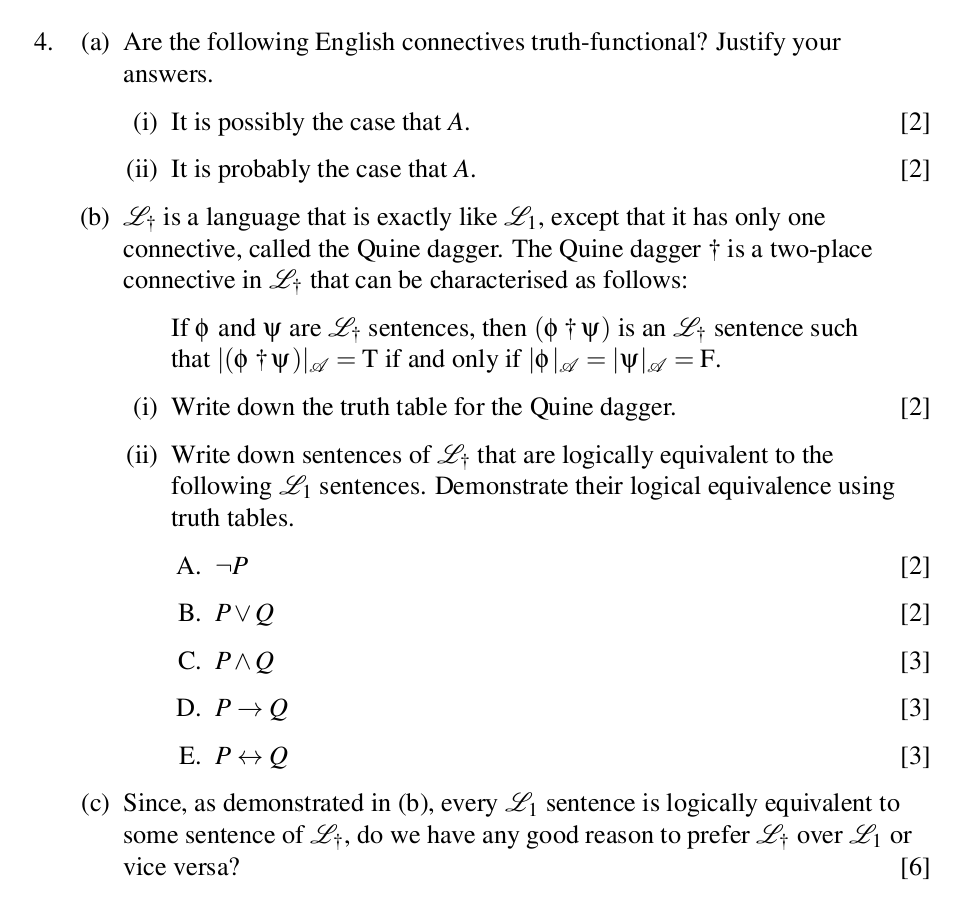
\includegraphics[width=1\textwidth]{Problem4.png}
\end{center}



\section*{Solutions}



















% \section*{TT2020: Problem 5}

% \begin{center}
%   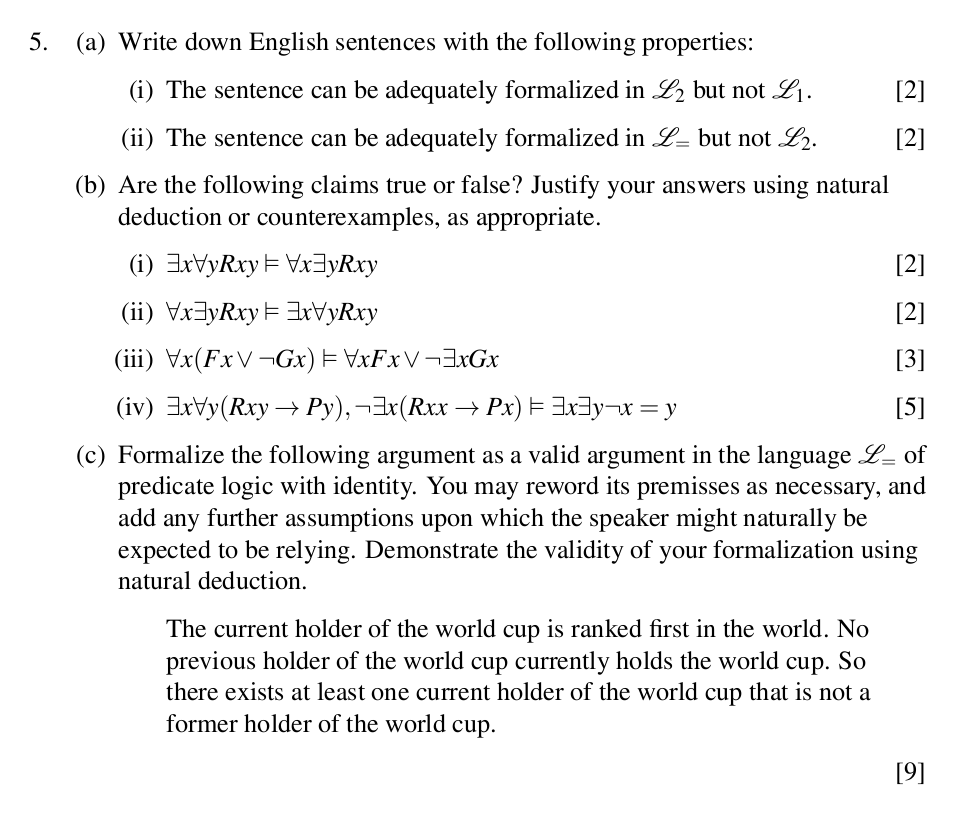
\includegraphics[width=1\textwidth]{Problem5.png}
% \end{center}



% \section*{Solutions}




% \vspace{.1in}
% \begin{customthm}{(5.a.i)}
%   The sentence can be formalised in $\mathscr{L}_2$ but not $\mathscr{L}_1$.
% \end{customthm}

% \begin{Answer}
%   In order of adequacy, consider the following answers:\\
%   (1) $P_1=$ `All men are mortal`.\\
%   (2) $P_2=$ `All cars owned by Sam are red`.\\ 
%   (3) $P_3\rightarrow P_4=$ `If Sam is a cat, then something is a cat`.
% \end{Answer}




% \vspace{.1in}
% \begin{customthm}{(5.a.ii)}
%   The sentence can be formalised in $\mathscr{L}_=$ but not $\mathscr{L}_2$.
% \end{customthm}

% \begin{Answer}
%   Earth has exactly one moon.
% \end{Answer}

% \newpage


% \vspace{.1in}
% \begin{customthm}{(5.b.i)}
%   $\exists x\forall y Rxy\vDash\forall x\exists y Rxy$.
% \end{customthm}

% \begin{Answer}
%   False.
%   Let $S=\set{1,2}$, $A$ be an $\mathscr{L}_2$ structure, and $a$ be a variable assignment in $A$ where $|R|_A=\set{\tuple{1,1},\tuple{1,2}}$ and $|x|_A^a=1$.
%   Letting $b$ be any variable assignment in $A$ differing at most in $y$ from $a$, it follows that $\tuple{|x|_A^b,|y|_A^b}\in|R|_A$.
%   Thus $|Rxy|_A=T$ for every variable assignment $b$ in $A$ differing at most in $y$, and so $|\forall y Rxy|_A^a=T$.
%   Thus $|\exists x\forall y Rxy|_A=T$.

%   We now let $c$ be a variable assignment in $A$ where $|x|_A^c=2$, observing that there is not $z\in S$ where $\tuple{|x|_A^c,z}\in|R|_A$, and so there is no variable assignment $d$ differing at most in $y$ from $c$ where $\tuple{|x|_A^d,|y|_A^d}\in|R|_A$. 
%   Thus $|Rxy|_A^d=F$ for all variable assignments $d$ which differ from $c$ at most in $y$, and so $|\exists y Rxy|_A^c=F$.
%   We may then conclude that $|\forall x\exists y Rxy|_A=F$, and so \textbf{5.b.i} fails to be valid.
% \end{Answer}






% \vspace{.1in}
% \begin{customthm}{(5.b.ii)}
%   $\forall x\exists y Rxy\vDash\exists x\forall y Rxy$.
% \end{customthm}

% \begin{Answer}
  
% \end{Answer}




% \vspace{.1in}
% \begin{customthm}{(5.b.iii)}
%   $\forall x(Fx\vee\neg Gx)\vDash\forall x Fx\vee\neg\exists xGx$
% \end{customthm}

% \begin{Answer}
  
% \end{Answer}





% \vspace{.1in}
% \begin{customthm}{(5.b.iv)}
%   $\exists x\forall y(Rxy\rightarrow Py),\ \neg\exists x(Rxx\rightarrow Px)\vDash\exists x\exists y\neg x=y$
% \end{customthm}

% \begin{Answer}
  
% \end{Answer}



\section*{Questions}

\vspace{.1in}
\begin{customthm}{(1)}
If $|Px|_A^a = T$, then there is a constant $k$ such that $|Pk|_A^a = T$.
\end{customthm}

\begin{Answer}
  % If seems intuitive that if $Px$ can be true, there must be a constant with the same value as $x$, but I’ve done questions before where this has not been the case. For example, $P: \set{1, 2, 3}, a=5, x=1$.
\end{Answer}








  % \begin{enumerate}[leftmargin=.5in,label=(\roman*)] 
  %     \item something
  %     \item somethin
  %   \end{enumerate}


\end{document}

